\documentclass{article}
\usepackage[UKenglish]{babel}% http://ctan.org/pkg/babel
\usepackage{graphicx}
\graphicspath{{images/}}

\usepackage{newspaper}
\date{\today}
\currentvolume{1}
\currentissue{1}
\usepackage{times}
\usepackage{graphicx}
\usepackage{multicol}

\SetPaperName{LVS today}
\SetHeaderName{LVS Ascot}
\SetPaperLocation{Ascot, Berkshire}
\SetPaperPrice{}
\SetPaperSlogan{LVS Ascot, founded in 1803 by the Licensed Trade Charity}
\usepackage{picinpar}
%uasage of picinpar:
%\begin{window}[1,l,\includegraphics{},caption]xxxxx\end{window}

%%%%%%%%%  Front matter   %%%%%%%%%%

\begin{document}
\maketitle

\begin{multicols}{3}{

\byline{\sc\Large A murder in Sarajevo}{Max Sepulveda}

\begin{window}[2,r,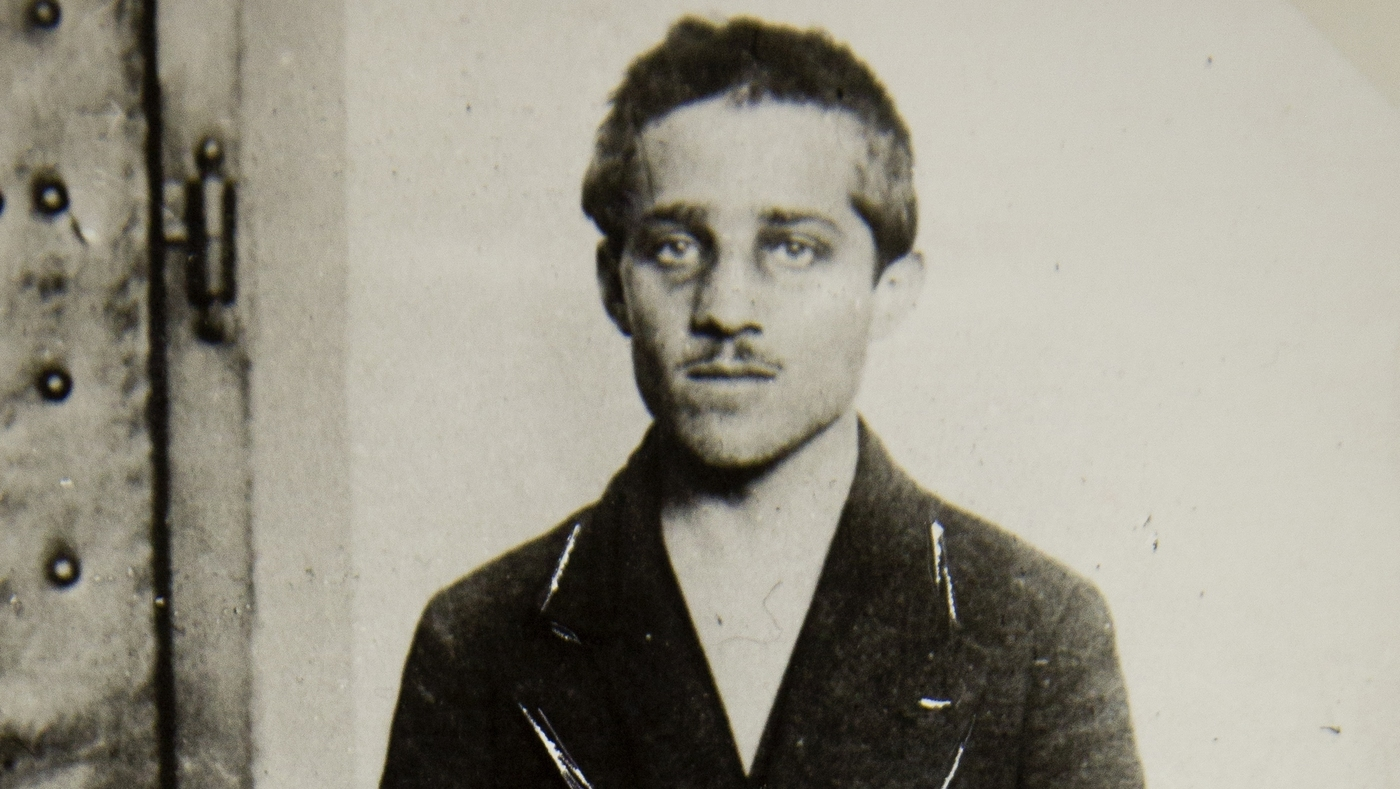
\includegraphics[width=2.3in]{killer},\centerline{Gavrilo Princip}] The assassination of Archduke Franz Ferdinand of Austria, heir presumptive to the Austro-Hungarian throne, and Franz Ferdinand's wife Sophie, Duchess of Hohenberg, occurred on 28 June 1914 in Sarajevo when they were mortally wounded by Gavrilo Princip. Princip was one of a group of six assassins (five Serbs and one Bosniak) coordinated by Danilo Ilić, a Bosnian Serb and a member of the Black Hand secret society. The political objective of the assassination was to break off Austria-Hungary's South Slav provinces so they could be combined into a Yugoslavia. The conspirators' motives were consistent with the movement that later became known as Young Bosnia. The assassination led directly to World War I when Austria-Hungary subsequently issued an ultimatum to the Kingdom of Serbia, which was partially rejected. Austria-Hungary then declared war on Serbia, triggering actions leading to war between most European states.

In charge of these Serbian military conspirators was Chief of Serbian Military Intelligence Dragutin Dimitrijević, his right-hand man Major Vojislav Tankosić, and the spy Rade Malobabić. Tankosić armed the assassins with bombs and pistols and trained them. The assassins were given access to the same clandestine network of safe-houses and agents that Malobabić used for the infiltration of weapons and operatives into Austria-Hungary.

\end{window}

\begin{window}[2,r,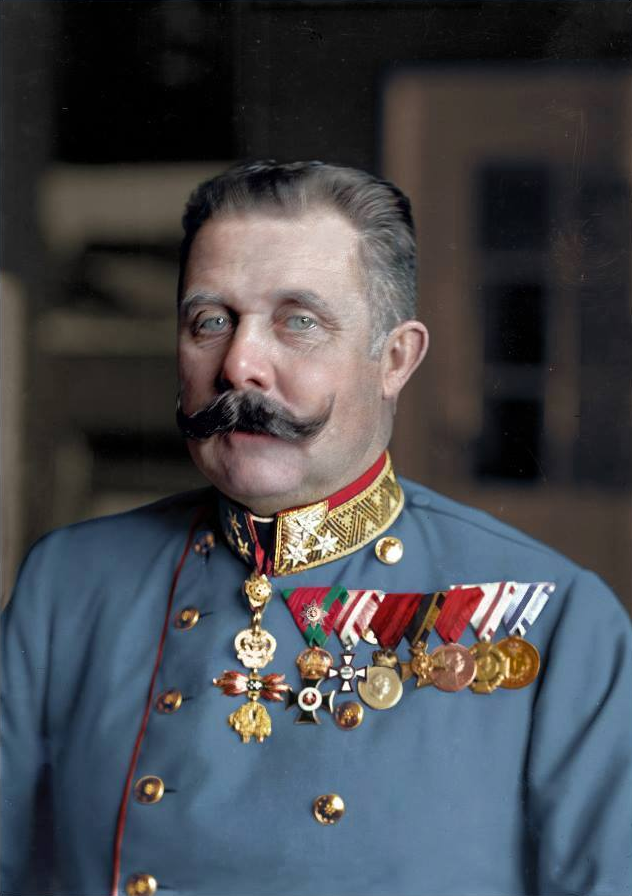
\includegraphics[width=1.5in]{archduke},\centerline{Archduke Franz Ferdinand}] The assassins, the key members of the clandestine network, and the key Serbian military conspirators who were still alive were arrested, tried, convicted and punished. Those who were arrested in Bosnia were tried in Sarajevo in October 1914. The other conspirators were arrested and tried before a Serbian court on the French-controlled Salonika Front in 1916–1917 on unrelated false charges; Serbia executed three of the top military conspirators. Much of what is known about the assassinations comes from these two trials and related records.

\end{window}
\closearticle


\headline{\it\huge Fire in Salem}
\begin{window}[2,r,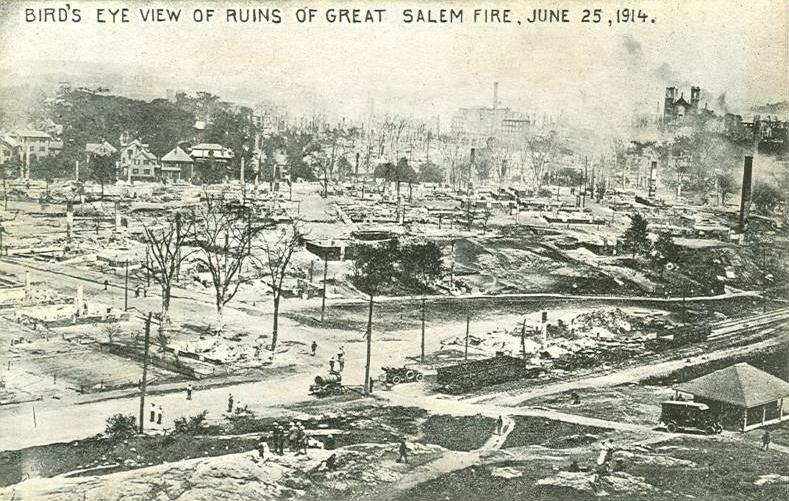
\includegraphics[width=1.5in]{Birds-eye_View_of_Ruins_of_Great_Salem_Fire},\centerline{Salem}] The Fire started with a series of explosions, caused by a mixture of acetone, amalacitate, alcohol, and celluloid. At 1:37 p.m. (EDT) on June 25, 1914, a fire alarm box was used to report a fire in the Korn Leather Factory at 57 Boston Street.

The fire spread quickly down and across Boston Street, due to a drought. The police department sent out calls to 21 cities for assistance. One industrial department, the Fore River Shipyard, also assisted. Over 90 out of town policemen came to help.


\end{window}

}
\end{multicols}

\end{document}